%----------------------------------------
% Write your notes here
%----------------------------------------

\definecolor{mygreen}{rgb}{0,0.6,0}
\definecolor{mygray}{rgb}{0.5,0.5,0.5}
\definecolor{mymauve}{rgb}{0.58,0,0.82}

\lstset{
  basicstyle=\ttfamily,
  columns=fullflexible,
  frame=single,
  breaklines=true,
  numbers=left,
  firstnumber=1,
  numberfirstline=true,
  backgroundcolor=\color{white},   % choose the background color
  commentstyle=\color{mygreen},    % comment style
  escapeinside={\%*}{*)},          % if you want to add LaTeX within your code
  keywordstyle=\color{blue},       % keyword style
  stringstyle=\color{mymauve},     % string literal style
}

\section{Computational Tractability}

Computational tractability is used to define whether an algorithm is practical or not with the current state of the art in computing. We need to trace how long an algorithm takes to run in terms of the input size (Note that input size does not always refer to number of inputs). Consider brute force cracking a password containing only 0s and 1s. This takes worst case $2^n$ tries where n is the length of the password. T(n) by convention is denotes the running time of an algorithm with input size n. This type of asymptotic analysis helps in a machine independent way of comparing algorithms based on the input size. A key assumption made is that comparison, indexing, arithmetic operations take constant time. A few general orders of T(n) are listed below :-
\begin{enumerate}
  \item Exponential T(n) = $k^n$ where k is a constant
  \item Polynomial T(n) = c$n^d$ where c, d are constants
  \item Linear T(n) = cn where c is a constant
  \item Logarithmic T(n) = logn
  \item Constant T(n) = c where c is a constant
\end{enumerate}
Note that logarithmic time algorithms will not look at all the data points even once. And constant time algorithms take the same time irrespective of the size of the input.
\\\\Note that there are a class of algorithms called pseudo-polynomial algorithm which does not depend on the number of inputs but rather the value of the input. Complex examples are the 0-1 Knapsack, Subset Sum problems. A more simple example is illustrated below. Here the algorithm has only one input. But the time the algorithm takes depends on the value of the input.
\begin{lstlisting}
def gotToZero(sum):
    while sum > 0:
        sum -= 1
\end{lstlisting}

\begin{figure}[H]
\centering
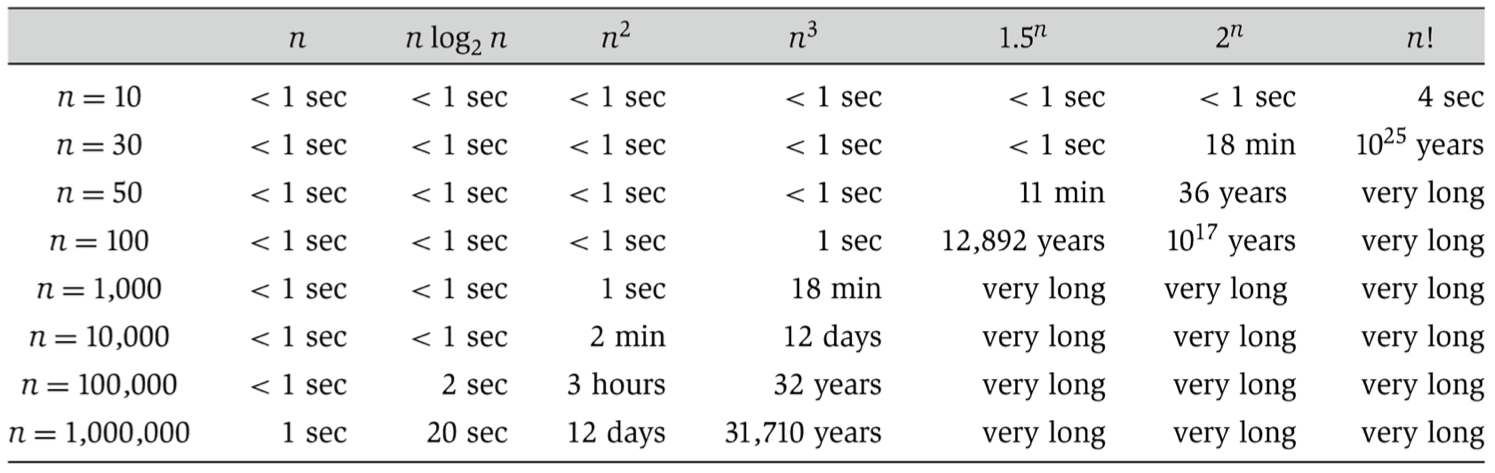
\includegraphics[scale=0.45]{figures/MDS4.png}
\caption{Table comparing input size with computation time}
    \label{fig:example_figure}
\end{figure}

\begin{figure}[H]
\centering
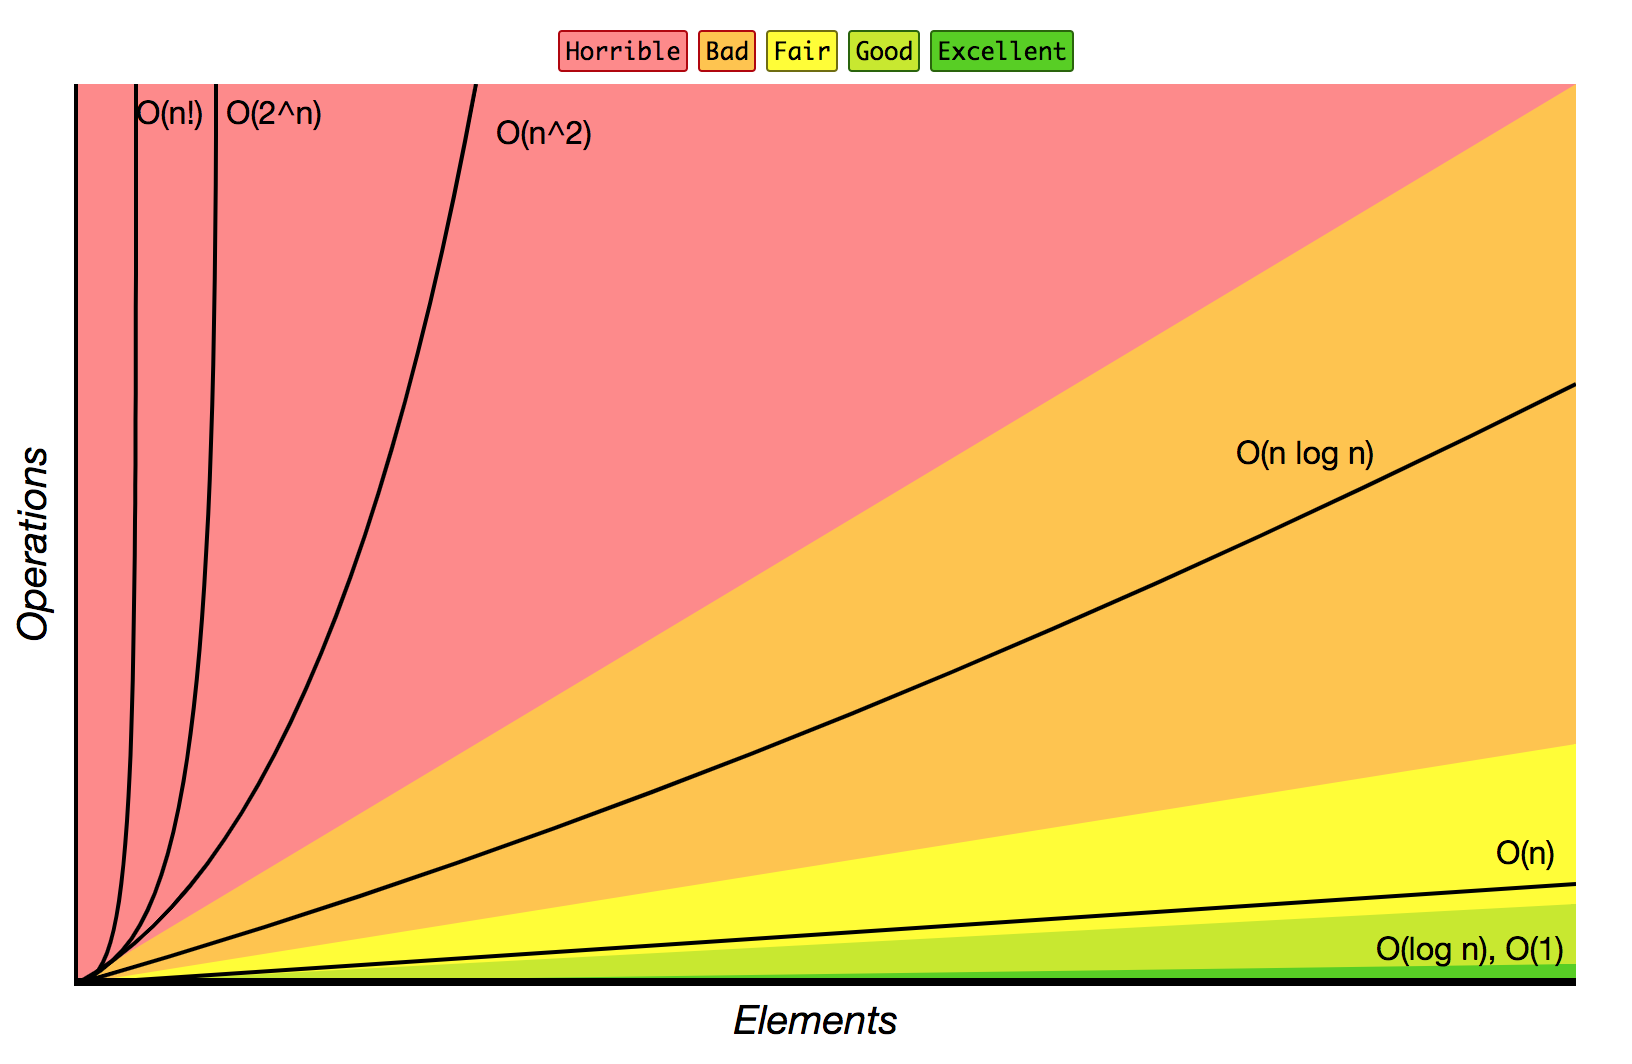
\includegraphics[scale=0.4]{figures/MDS1.png}
\caption{Graph depicting orders of growth \href{http://bigocheatsheet.com/}{Reference Link}}
    \label{fig:example_figure}
\end{figure}



\section{Analysis of Runtime}
Note that the algorithm will not the same time for all types of inputs even if the values are same.
\begin{enumerate}
  \item Worst Case : In the worst case analysis, we calculate upper bound on running time of an algorithm which stands for that input which causes the maximum number of operations to be executed. For example, in the case of linear search, the worst case input is when the element we are searching for is in the last position. So worst case T(n) = n.
  \item Average Case : In average case analysis, take all possible inputs and calculate computing time for all of the inputs. Sum all the calculated values and divide the sum by total number of inputs. For the simple linear search example, the various inputs are the inputs where the key element to be searched are in the different places in the array. Average Case T(n) = $\frac{1}{n} \sum_{i=1}^{n} i $.
  \item Best Case : In best case analysis, we try to find the input which causes the minimum number of operations. For the simple linear search example, the best case input happens is when the element we are searching for is in the first position. So best case T(n) = 1.
  \item Amortized : Amortized analysis is used for algorithms where an occasional operation is very slow, but most of the other operations are faster. In Amortized Analysis, we analyze a sequence of operations and guarantee a worst case average time which is lower than the worst case time of a particular expensive operation. Consider a problem of simple insertions into a dynamic size array.
  Initially size of array is 0. When an insertion occurs, overflow happens, array size is expanded to 1. When another insertion occurs, overflow happens, array size is doubled to 2 and so on. The algorithm and analysis is explained in Figure 2 and Figure 3. Reference : \href{https://www.geeksforgeeks.org/analysis-algorithm-set-5-amortized-analysis-introduction/}{Link}
  
\end{enumerate}
Note that typically worst case and average case of algorithms are taken into consideration and not the best case because there is no practical use of best case analysis.

\begin{figure}[H]
\centering
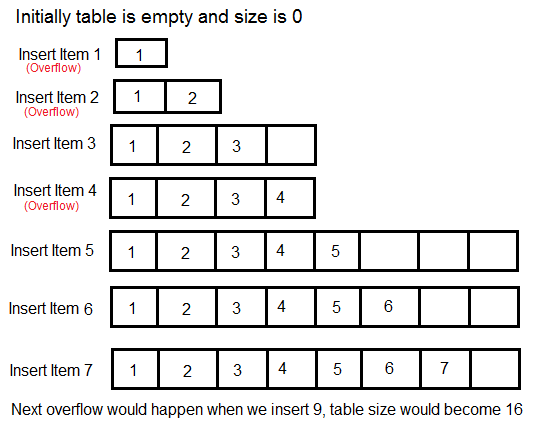
\includegraphics[scale=0.6]{figures/MDS2.png}
\caption{Example of dynamic table}
    \label{fig:example_figure}
\end{figure}

\begin{figure}[H]
\centering
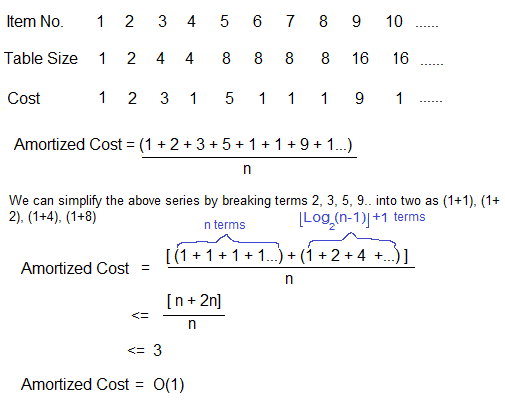
\includegraphics[scale=0.6]{figures/MDS3.png}
\caption{Dynamic table complexity analyis}
    \label{fig:example_figure}
\end{figure}

\section{Orders of Growth}
For easier comparison of algorithms, we approximate T(n) by orders of growth. We consider only the dominant term of T(n), since the lower-order terms are relatively insignificant for large values of n. We also ignore the dominant term's constant coefficient, since constant factors are less significant than the rate of growth in determining computational efficiency for large inputs. An algorithm is typically "considered" to be more time efficient than another if its worst case
running time has a lower order of growth. However, note that due to constant factors and lower order terms, an algorithm whose running time has a higher order of growth might take less time for small inputs than an algorithm whose running time has a lower order of growth.

\subsection{Big-Oh : Upper Bound}
O(g(n)) = { f(n) $| \exists$ $\constant$ c $>$ 0 and $n_0$ such that $\forall$ n $\geq$ $n_0$ : $0 \leq f(n) \leq cg(n)$ }
\\\\Example :-
\[ T(n) = 32n^2 + 17n + 1 \]
\[ T(n) = O(n^3) \]

\begin{figure}[H]
\centering
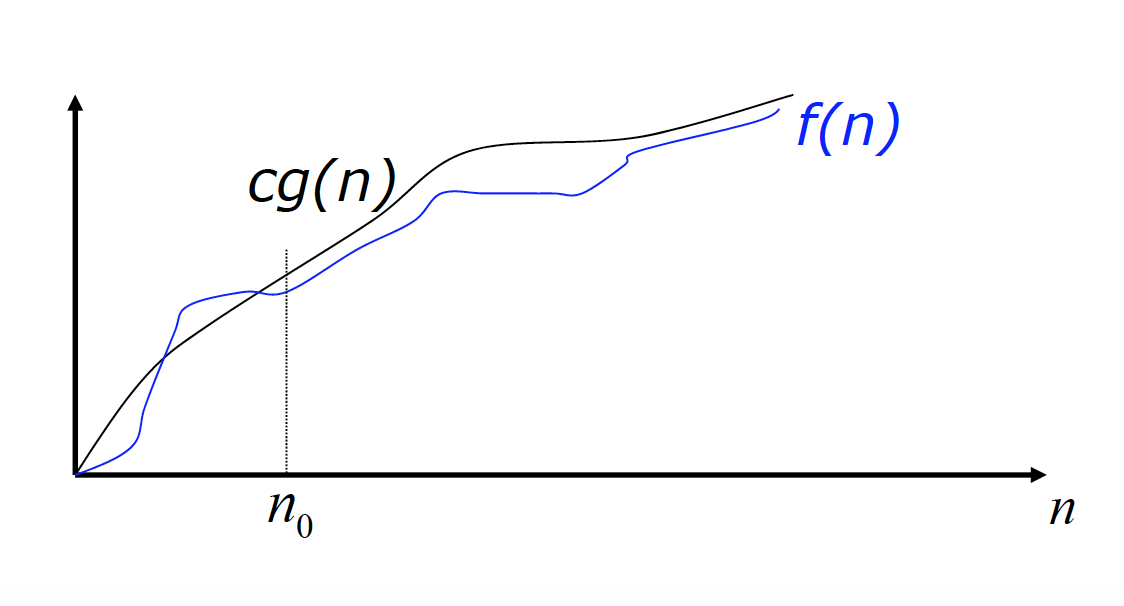
\includegraphics[scale=0.6]{figures/MDS5.png}
\caption{Big-Oh graph}
    \label{fig:example_figure}
\end{figure}

\subsection{Big-Omega : Lower Bound}
$\Omega$(g(n)) = { f(n) $| \exists$ $\constant$ c $>$ 0 and $n_0$ such that $\forall$ n $\geq$ $n_0$ : $0 \leq f(n) \leq cg(n)$ }
\\\\Example :-
\[ T(n) = 32n^2 + 17n + 1 \]
\[ T(n) = O(n) \]

\begin{figure}[H]
\centering
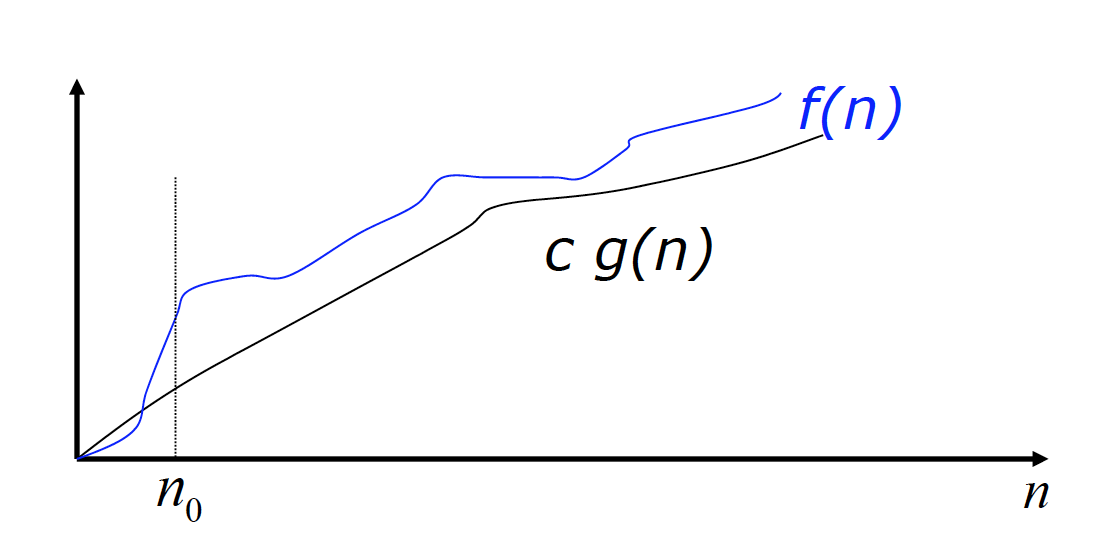
\includegraphics[scale=0.6]{figures/MDS6.png}
\caption{Big-Omega graph}
    \label{fig:example_figure}
\end{figure}

\subsection{Big-Theta : Tight Bound}
$\Theta$(g(n)) = { f(n) $| \exists$ $\constants$ c1, c2 $>$ 0 and $n_0$ such that $\forall$ n $\geq$ $n_0$ : $c1g(n) \leq f(n) \leq c2g(n)$ }
\\\\Example :-
\[ T(n) = 5n^2 + 17n + 1 \]
\[ T(n) = \Theta(n^2) \]

\begin{figure}[H]
\centering
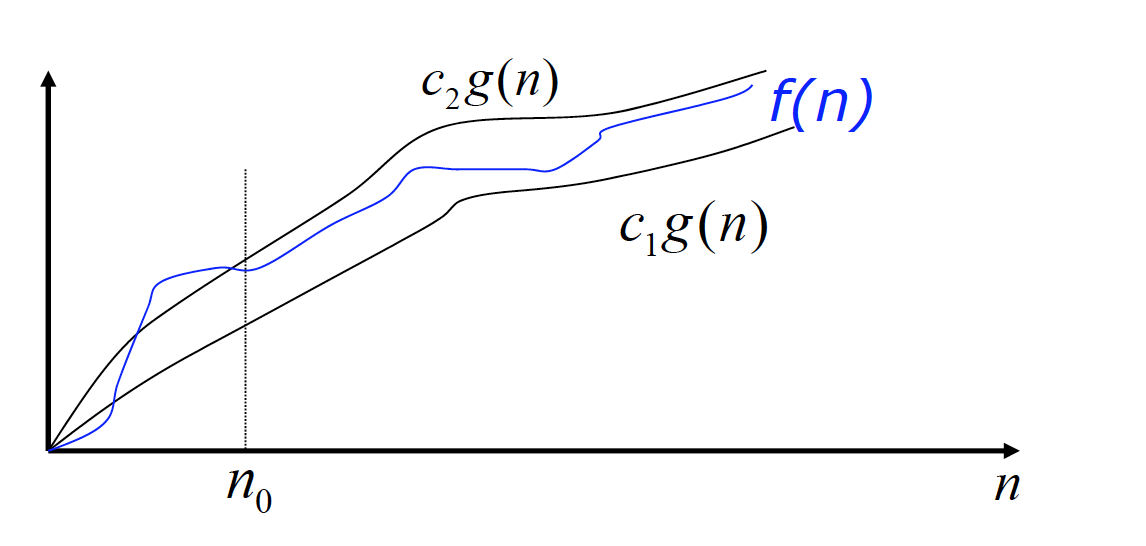
\includegraphics[scale=0.6]{figures/MDS7.png}
\caption{Big-Theta graph}
    \label{fig:example_figure}
\end{figure}

\subsection{Little-Oh}
o(g(n)) = { f(n) $|  $\forall$ $\constant$ c $>$ 0 \exists$ $n_0$ such that $\forall$ n $\geq$ $n_0$ : $0 \leq f(n) \leq cg(n)$ }
f(n) = o(g(n)) means that for large n, function f is smaller
than any constant fraction of g
\\\\Example :-
\[ T(n) = 5n \]
\[ T(n) = o(n^2) \]
\[ T(n) \neq o(n) \]

\subsection{Little-Omega}
$\omega$(g(n)) = { f(n) $|  $\forall$ $\constant$ c $>$ 0 \exists$ $n_0$ such that $\forall$ n $\geq$ $n_0$ : $0 \leq cg(n) \leq f(n) $ }
f(n) = $\omega$(g(n)) means that for large n, function f is larger than
any constant multiple of g
\\\\Example :-
\[ T(n) = 5n^2 \]
\[ T(n) = \omega(n) \]
\[ T(n) = \omega(n^2) \]

\begin{figure}[H]
\centering
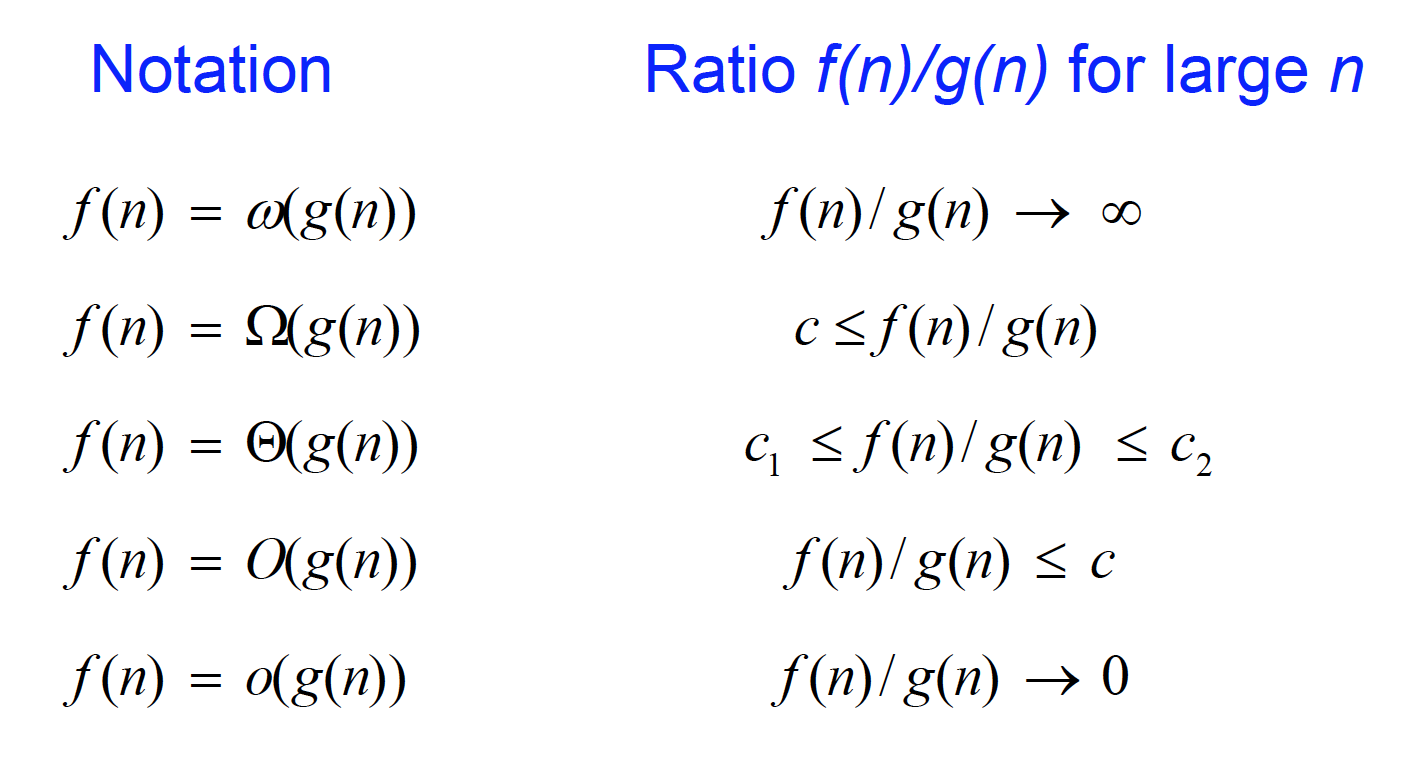
\includegraphics[scale=0.35]{figures/MDS8.png}
\caption{Summary of asymptotic analysis}
    \label{fig:example_figure}
\end{figure}

\subsection{A few rules of thumb}

\begin{enumerate}
    \item 
    \[ T(n) = a_0 + a_1 n + .... + a_d n^d \]
    \[ T(n) = O(n^d) \]
    \[ T(n) = O(n^d) \]
    \[ T(n) = O(n^d) \]
    
    \item 
    \[ T(n) = log_a(n) \]
    \[ T(n) = O(\frac{log_b(n)}{log_b(a)}) \]
    \[ T(n) = O(log_b(a)) \text{ } \forall \text{ } a, b > 0 \]
    
    \item 
    \[ T(n) = n^d \]
    \[ T(n) = O(r^n) \text{ } \forall \text{ } r > 1, d > 0 \]

\end{enumerate}



\section{Common Running Times}

\subsection{Linear Time}
Examples : Finding an element (Linear Search), Finding minimum, Finding maximum
\\\\Note that insertion into a linked list is not a linear time algorithm because in addition to maintaining a head, we also maintain a tail and insert values at the end and hence a constant time algorithm.
\\\\Insertion into a linked list at a specific position need not be a linear time because we can maintain a hash table where key is the index and value is the pointer to the node at index/position in the linked list. Now insertion will take O(1) time. However, this takes O(n) space. Designing algorithms is typically a trade-off between space complexity and time complexity. 

\subsection{Logarithmic Time}
Examples : Balanced Binary Search Tree - Search and Insert. Binary Search on a sorted array.
\\\\In binary search on a sorted array, we look at the middle element and compare it to the element we are searching for, and hence reduce search space by half for each comparison we make. Therefore in the worst case we take logn time to find the element.
\\\\Skip lists is a probabilistic data structure built on top of linked lists with O(log(n)) search and O(n) space. Refer \href{https://brilliant.org/wiki/skip-lists/}{here} for more information.

\subsection{Linearithmic Time - O(nlogn)}
Examples : Quick Sort Average Case
\\\\In quick sort, the algorithm picks a pivot element and partitions the array based on the pivot so that elements lesser than the pivot come to the left of the pivot and elements greater then the pivot to the right. This is done recursively on the left and the right till the whole array is sorted. So in the best case, the pivot chosen will always be the middle position elements of the subarray. This leads to O(n) work being done on each level while the array size gets halved every level. Therefore, O(nlogn) time complexity in the best case. Average case (using percentile analysis) is the 1/4 and 3/4 partition which gives again O(nlogn) time complexity.

\subsection{Polynomial - O($n^2$)}
Examples : Bubble Sort, Quick Sort Worst Case
\\\\In bubble sort, we do all pairs comparison. That is the algorithm takes approx O(n) per element. Since there are n elements, bubble sort takes O($n^2$) time.
\\\\In the worst case of quicksort, the pivot picked is always the greatest of smallest element of the subarray. This gives us the recurrence T(n) = O(n) + T(n-1) which gives us T(n) = O($n^2$).


\section{Applications}

\subsection{Lower Bound}
An application of lower bound analysis is during algorithm design when there is a formal proof that you can do no better than then lower bound during optimization. An example is the formal proof outlined in \href{https://www.cs.cmu.edu/~avrim/451f11/lectures/lect0913.pdf}{this paper} for comparison based sorting algorithms to have a lower bound of nlogn for average case.

\subsection{Join}
Consider that we have two tables T1 and T2 with columns id, A, B and id, C, D respectively. Supposed if we wanted to join theses two tables to get id, A, B, C, D. One way to accomplish this would be for every element in A run through every element in B to find the rows of B with matching ids. This would take $O(n^2)$ time. A better approach would be to sort the table T2 and for each id in T1 do a binary serach to find the first occurance of id. This would take approximate O(nlogn) for sorting T2 and O(nlogn) for the joining process which results in O(nlogn). The idea is illustrated \href{https://en.wikipedia.org/wiki/Sort-merge_join}{here}. Another approach would be to iterate through T1 and put all the rows into a hash table indexed by the id. Now for each row in T2, just refer to the hash table by id to get the rows of T1 with the same id. This takes O(n) time. A detailed explanation is provided \href{https://en.wikipedia.org/wiki/Hash_join}{here}.

\subsection{Universal Data Structure}
Consider a wordload with inserts followed by lookups followed by range queries. The task is to come up with a data structure that is best suited for the workload. From earlier analysis, linked list would be the best for the insert phase with O(1) time. For the lookup phase, hashmaps would be ideal with O(1) lookup. For range queries, trees would give good performance. However, there is no known data structure that would perform best in all three phases. There is research going on to design a data structure that would perform good in all three phases maybe using morphing.